%%%%% 2-entities Diffie-Hellman
\subsection*{a) Traditional Diffie-Hellman key exchange protocol}
%
Two parties participate in the protocol: Alice (A) and Bob (B).
\begin{itemize}
    \item Alice and Bob agree to use the publicly known prime \(p\) and
    the generator \(g\).
    \item Alice selects a secret number \(a\) and then sends to Bob \(A=g^a \mod p\).
    \item Bob also selects a secret number \(b\) and then sends to Alice \(B=g^b \mod p\).
    \item Alice computes \(s=B^a \mod p\).
    \item Bob computes \(s=A^b \mod p\).
    \item At this point, they both share the common key \(s=g^{ab} \mod p\).
\end{itemize}

\begin{figure}
    \centering
    \tikzset{every picture/.style={line width=0.75pt}} %set default line width to 0.75pt        

    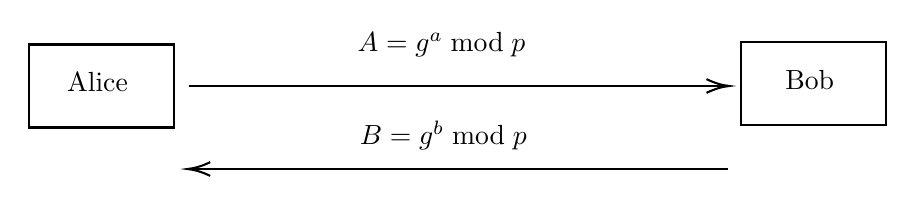
\begin{tikzpicture}[x=0.75pt,y=0.75pt,yscale=-1,xscale=1]
    %uncomment if require: \path (0,114); %set diagram left start at 0, and has height of 114

    %Shape: Rectangle [id:dp8876548329540627] 
    \draw   (123,21) -- (193,21) -- (193,61) -- (123,61) -- cycle ;

    %Shape: Rectangle [id:dp3410651517379072] 
    \draw   (466,20) -- (536,20) -- (536,60) -- (466,60) -- cycle ;

    %Straight Lines [id:da2693979433068405] 
    \draw    (200,41) -- (458.5,41) ;
    \draw [shift={(460.5,41)}, rotate = 180] [color={rgb, 255:red, 0; green, 0; blue, 0 }  ][line width=0.75]    (10.93,-3.29) .. controls (6.95,-1.4) and (3.31,-0.3) .. (0,0) .. controls (3.31,0.3) and (6.95,1.4) .. (10.93,3.29)   ;
    %Straight Lines [id:da7762422493799963] 
    \draw    (460,81) -- (201.5,81) ;
    \draw [shift={(199.5,81)}, rotate = 360] [color={rgb, 255:red, 0; green, 0; blue, 0 }  ][line width=0.75]    (10.93,-3.29) .. controls (6.95,-1.4) and (3.31,-0.3) .. (0,0) .. controls (3.31,0.3) and (6.95,1.4) .. (10.93,3.29)   ;

    % Text Node
    \draw (140,33) node [anchor=north west][inner sep=0.75pt]   [align=left] {Alice};
    % Text Node
    \draw (486,32) node [anchor=north west][inner sep=0.75pt]   [align=left] {Bob};
    % Text Node
    \draw (280,13.4) node [anchor=north west][inner sep=0.75pt]    {$A=g^{a}\bmod p$};
    % Text Node
    \draw (281,56.4) node [anchor=north west][inner sep=0.75pt]    {$B=g^{b}\bmod p$};
    \end{tikzpicture}
    \caption{2-parties DH key exchange.(Exercise 4)}\label{fig:2_DH}

\end{figure}

Visualization of the protocol in \autoref{fig:2_DH}.

%%%%% 3-entities Diffie-Hellman
\subsection*{b) Three--party Diffie-Hellman}
%
Three parties participate in the protocol: Alice (A), Bob (B), and Carol (C).
\begin{itemize}
    \item Alice, Bob, and Carol agree on use the publicly known prime \(p\) and
    the generator \(g\).
    \item ROUND 1:
    \begin{itemize}
        \item Alice selects a secret number \(a\) and then sends to Bob \(A=g^a \mod p\).
        \item Bob selects a secret number \(b\) and then sends to Carol \(B=g^b \mod p\).
        \item Carol selects a secret number \(c\) and then sends to Alice \(C=g^c \mod p\).
    \end{itemize}
    \item ROUND 2:
    \begin{itemize}
        \item Alice computes \(A_C=C^a \mod p=g^{ca} \mod p\) and sends to Bob.
        \item Bob computes \(B_A=A^b \mod p=g^{ab} \mod p\) and sends to Carol.
        \item Carol computes \(C_B=B^c \mod p=g^{bc} \mod p\) and sends to Alice.
    \end{itemize}
    \item Alice computes \(s=C_B^a \mod p=g^{bca} \mod p\).
    \item Bob computes \(s=A_C^b \mod p=g^{cab} \mod p\).
    \item Carol computes \(s=B_A^c \mod p=g^{abc} \mod p\).
    \item At this point, they share the common key \(s=g^{abc} \mod p\).
\end{itemize}

Visualization of the protocol in \autoref{fig:3_DH}.

\begin{figure}[!hpt]
    \centering
    \tikzset{every picture/.style={line width=0.75pt}} %set default line width to 0.75pt        

    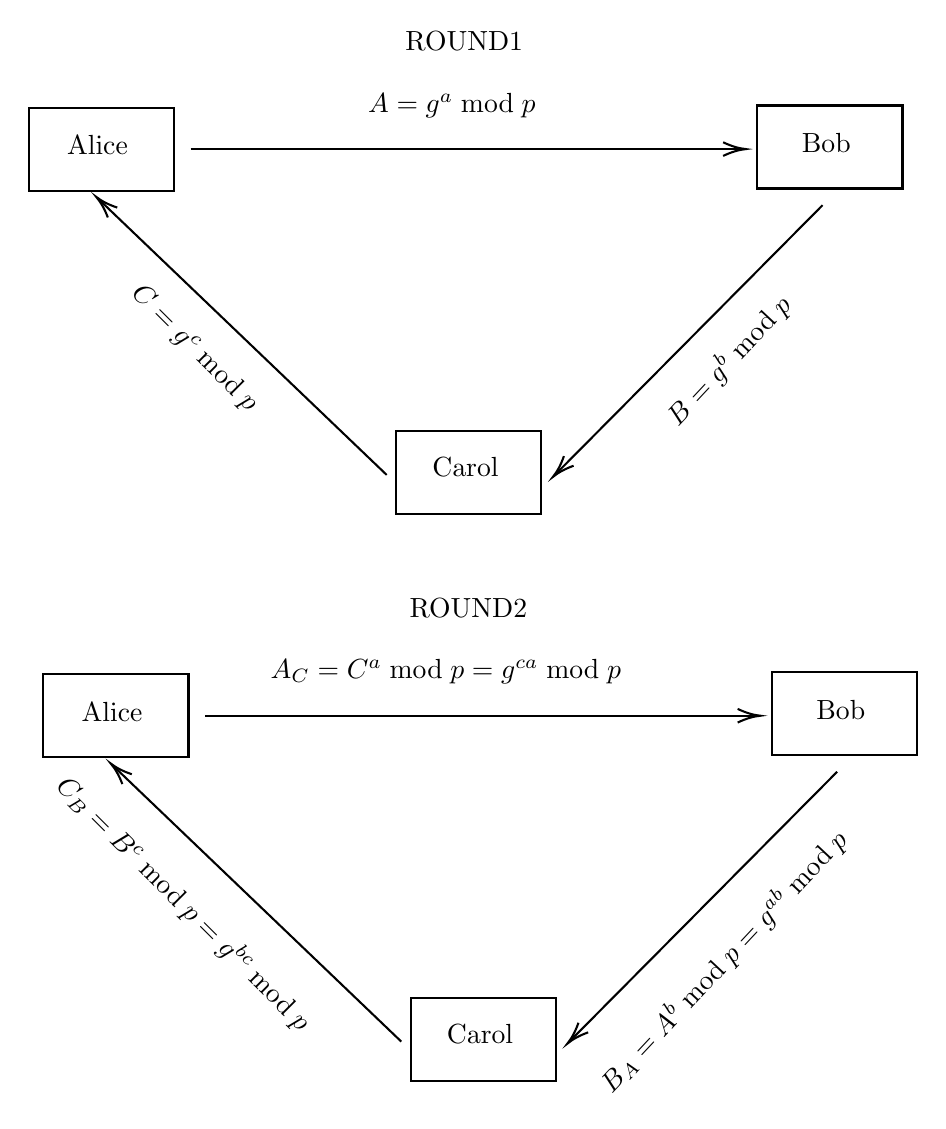
\begin{tikzpicture}[x=0.75pt,y=0.75pt,yscale=-1,xscale=1]
    %uncomment if require: \path (0,611); %set diagram left start at 0, and has height of 611

    %Shape: Rectangle [id:dp4537349834049913] 
    \draw   (121,48) -- (191,48) -- (191,88) -- (121,88) -- cycle ;

    %Shape: Rectangle [id:dp9368486843549375] 
    \draw   (472,47) -- (542,47) -- (542,87) -- (472,87) -- cycle ;

    %Shape: Rectangle [id:dp5642407598491361] 
    \draw   (298,204) -- (368,204) -- (368,244) -- (298,244) -- cycle ;

    %Straight Lines [id:da02137938109829618] 
    \draw    (199,68) -- (464.5,68) ;
    \draw [shift={(466.5,68)}, rotate = 180] [color={rgb, 255:red, 0; green, 0; blue, 0 }  ][line width=0.75]    (10.93,-3.29) .. controls (6.95,-1.4) and (3.31,-0.3) .. (0,0) .. controls (3.31,0.3) and (6.95,1.4) .. (10.93,3.29)   ;
    %Straight Lines [id:da9261004491801275] 
    \draw    (503.5,95) -- (374.91,224.58) ;
    \draw [shift={(373.5,226)}, rotate = 314.78] [color={rgb, 255:red, 0; green, 0; blue, 0 }  ][line width=0.75]    (10.93,-3.29) .. controls (6.95,-1.4) and (3.31,-0.3) .. (0,0) .. controls (3.31,0.3) and (6.95,1.4) .. (10.93,3.29)   ;
    %Straight Lines [id:da9096770241098924] 
    \draw    (293.5,225) -- (154.94,92.38) ;
    \draw [shift={(153.5,91)}, rotate = 43.75] [color={rgb, 255:red, 0; green, 0; blue, 0 }  ][line width=0.75]    (10.93,-3.29) .. controls (6.95,-1.4) and (3.31,-0.3) .. (0,0) .. controls (3.31,0.3) and (6.95,1.4) .. (10.93,3.29)   ;
    %Shape: Rectangle [id:dp7358041674397383] 
    \draw   (128,321) -- (198,321) -- (198,361) -- (128,361) -- cycle ;

    %Shape: Rectangle [id:dp9251010892536913] 
    \draw   (479,320) -- (549,320) -- (549,360) -- (479,360) -- cycle ;

    %Shape: Rectangle [id:dp8135789420174808] 
    \draw   (305,477) -- (375,477) -- (375,517) -- (305,517) -- cycle ;

    %Straight Lines [id:da3374021317133087] 
    \draw    (206,341) -- (471.5,341) ;
    \draw [shift={(473.5,341)}, rotate = 180] [color={rgb, 255:red, 0; green, 0; blue, 0 }  ][line width=0.75]    (10.93,-3.29) .. controls (6.95,-1.4) and (3.31,-0.3) .. (0,0) .. controls (3.31,0.3) and (6.95,1.4) .. (10.93,3.29)   ;
    %Straight Lines [id:da09585275791462244] 
    \draw    (510.5,368) -- (381.91,497.58) ;
    \draw [shift={(380.5,499)}, rotate = 314.78] [color={rgb, 255:red, 0; green, 0; blue, 0 }  ][line width=0.75]    (10.93,-3.29) .. controls (6.95,-1.4) and (3.31,-0.3) .. (0,0) .. controls (3.31,0.3) and (6.95,1.4) .. (10.93,3.29)   ;
    %Straight Lines [id:da6087337836699833] 
    \draw    (300.5,498) -- (161.94,365.38) ;
    \draw [shift={(160.5,364)}, rotate = 43.75] [color={rgb, 255:red, 0; green, 0; blue, 0 }  ][line width=0.75]    (10.93,-3.29) .. controls (6.95,-1.4) and (3.31,-0.3) .. (0,0) .. controls (3.31,0.3) and (6.95,1.4) .. (10.93,3.29)   ;

    % Text Node
    \draw (283,39.4) node [anchor=north west][inner sep=0.75pt]    {$A=g^{a}\bmod p$};
    % Text Node
    \draw (423.56,194.63) node [anchor=north west][inner sep=0.75pt]  [rotate=-313.1]  {$B=g^{b}\bmod p$};
    % Text Node
    \draw (492,59) node [anchor=north west][inner sep=0.75pt]   [align=left] {Bob};
    % Text Node
    \draw (138,60) node [anchor=north west][inner sep=0.75pt]   [align=left] {Alice};
    % Text Node
    \draw (314,215) node [anchor=north west][inner sep=0.75pt]   [align=left] {Carol};
    % Text Node
    \draw (176.68,129.6) node [anchor=north west][inner sep=0.75pt]  [rotate=-44.93]  {$C=g^{c}\bmod p$};
    % Text Node
    \draw (236,312.4) node [anchor=north west][inner sep=0.75pt]    {$A_{C} =C^{a}\bmod p=g^{ca}\bmod p$};
    % Text Node
    \draw (391.56,515.63) node [anchor=north west][inner sep=0.75pt]  [rotate=-313.1]  {$B_{A} =A^{b}\bmod p=g^{ab}\bmod p$};
    % Text Node
    \draw (141.68,365.6) node [anchor=north west][inner sep=0.75pt]  [rotate=-44.93]  {$C_{B} =B^{c}\bmod p=g^{bc}\bmod p$};
    % Text Node
    \draw (321,488) node [anchor=north west][inner sep=0.75pt]   [align=left] {Carol};
    % Text Node
    \draw (499,332) node [anchor=north west][inner sep=0.75pt]   [align=left] {Bob};
    % Text Node
    \draw (145,333) node [anchor=north west][inner sep=0.75pt]   [align=left] {Alice};
    % Text Node
    \draw (301,10) node [anchor=north west][inner sep=0.75pt]   [align=left] {ROUND1};
    % Text Node
    \draw (303,283) node [anchor=north west][inner sep=0.75pt]   [align=left] {ROUND2};
    \end{tikzpicture}
    \caption{3-parties DH key exchange.(Exercise 4)}\label{fig:3_DH}

\end{figure}